% GNUPLOT: LaTeX picture with Postscript
\begingroup
  \makeatletter
  \providecommand\color[2][]{%
    \GenericError{(gnuplot) \space\space\space\@spaces}{%
      Package color not loaded in conjunction with
      terminal option `colourtext'%
    }{See the gnuplot documentation for explanation.%
    }{Either use 'blacktext' in gnuplot or load the package
      color.sty in LaTeX.}%
    \renewcommand\color[2][]{}%
  }%
  \providecommand\includegraphics[2][]{%
    \GenericError{(gnuplot) \space\space\space\@spaces}{%
      Package graphicx or graphics not loaded%
    }{See the gnuplot documentation for explanation.%
    }{The gnuplot epslatex terminal needs graphicx.sty or graphics.sty.}%
    \renewcommand\includegraphics[2][]{}%
  }%
  \providecommand\rotatebox[2]{#2}%
  \@ifundefined{ifGPcolor}{%
    \newif\ifGPcolor
    \GPcolortrue
  }{}%
  \@ifundefined{ifGPblacktext}{%
    \newif\ifGPblacktext
    \GPblacktexttrue
  }{}%
  % define a \g@addto@macro without @ in the name:
  \let\gplgaddtomacro\g@addto@macro
  % define empty templates for all commands taking text:
  \gdef\gplbacktext{}%
  \gdef\gplfronttext{}%
  \makeatother
  \ifGPblacktext
    % no textcolor at all
    \def\colorrgb#1{}%
    \def\colorgray#1{}%
  \else
    % gray or color?
    \ifGPcolor
      \def\colorrgb#1{\color[rgb]{#1}}%
      \def\colorgray#1{\color[gray]{#1}}%
      \expandafter\def\csname LTw\endcsname{\color{white}}%
      \expandafter\def\csname LTb\endcsname{\color{black}}%
      \expandafter\def\csname LTa\endcsname{\color{black}}%
      \expandafter\def\csname LT0\endcsname{\color[rgb]{1,0,0}}%
      \expandafter\def\csname LT1\endcsname{\color[rgb]{0,1,0}}%
      \expandafter\def\csname LT2\endcsname{\color[rgb]{0,0,1}}%
      \expandafter\def\csname LT3\endcsname{\color[rgb]{1,0,1}}%
      \expandafter\def\csname LT4\endcsname{\color[rgb]{0,1,1}}%
      \expandafter\def\csname LT5\endcsname{\color[rgb]{1,1,0}}%
      \expandafter\def\csname LT6\endcsname{\color[rgb]{0,0,0}}%
      \expandafter\def\csname LT7\endcsname{\color[rgb]{1,0.3,0}}%
      \expandafter\def\csname LT8\endcsname{\color[rgb]{0.5,0.5,0.5}}%
    \else
      % gray
      \def\colorrgb#1{\color{black}}%
      \def\colorgray#1{\color[gray]{#1}}%
      \expandafter\def\csname LTw\endcsname{\color{white}}%
      \expandafter\def\csname LTb\endcsname{\color{black}}%
      \expandafter\def\csname LTa\endcsname{\color{black}}%
      \expandafter\def\csname LT0\endcsname{\color{black}}%
      \expandafter\def\csname LT1\endcsname{\color{black}}%
      \expandafter\def\csname LT2\endcsname{\color{black}}%
      \expandafter\def\csname LT3\endcsname{\color{black}}%
      \expandafter\def\csname LT4\endcsname{\color{black}}%
      \expandafter\def\csname LT5\endcsname{\color{black}}%
      \expandafter\def\csname LT6\endcsname{\color{black}}%
      \expandafter\def\csname LT7\endcsname{\color{black}}%
      \expandafter\def\csname LT8\endcsname{\color{black}}%
    \fi
  \fi
    \setlength{\unitlength}{0.0500bp}%
    \ifx\gptboxheight\undefined%
      \newlength{\gptboxheight}%
      \newlength{\gptboxwidth}%
      \newsavebox{\gptboxtext}%
    \fi%
    \setlength{\fboxrule}{0.5pt}%
    \setlength{\fboxsep}{1pt}%
\begin{picture}(9060.00,6800.00)%
    \gplgaddtomacro\gplbacktext{%
      \csname LTb\endcsname%
      \put(830,3791){\makebox(0,0)[r]{\strut{}$10^{-1}$}}%
      \csname LTb\endcsname%
      \put(830,4314){\makebox(0,0)[r]{\strut{}$10^{0}$}}%
      \csname LTb\endcsname%
      \put(830,4837){\makebox(0,0)[r]{\strut{}$10^{1}$}}%
      \csname LTb\endcsname%
      \put(830,5361){\makebox(0,0)[r]{\strut{}$10^{2}$}}%
      \csname LTb\endcsname%
      \put(830,5884){\makebox(0,0)[r]{\strut{}$10^{3}$}}%
      \csname LTb\endcsname%
      \put(830,6407){\makebox(0,0)[r]{\strut{}$10^{4}$}}%
      \csname LTb\endcsname%
      \put(932,3612){\makebox(0,0){\strut{}$10^{2}$}}%
      \csname LTb\endcsname%
      \put(2117,3612){\makebox(0,0){\strut{}$10^{3}$}}%
      \csname LTb\endcsname%
      \put(3302,3612){\makebox(0,0){\strut{}$10^{4}$}}%
      \csname LTb\endcsname%
      \put(4487,3612){\makebox(0,0){\strut{}$10^{5}$}}%
      \csname LTb\endcsname%
      \put(5672,3612){\makebox(0,0){\strut{}$10^{6}$}}%
      \csname LTb\endcsname%
      \put(6857,3612){\makebox(0,0){\strut{}$10^{7}$}}%
      \csname LTb\endcsname%
      \put(6959,3791){\makebox(0,0)[l]{\strut{} }}%
      \csname LTb\endcsname%
      \put(6959,4314){\makebox(0,0)[l]{\strut{} }}%
      \csname LTb\endcsname%
      \put(6959,4837){\makebox(0,0)[l]{\strut{} }}%
      \csname LTb\endcsname%
      \put(6959,5361){\makebox(0,0)[l]{\strut{} }}%
      \csname LTb\endcsname%
      \put(6959,5884){\makebox(0,0)[l]{\strut{} }}%
      \csname LTb\endcsname%
      \put(6959,6407){\makebox(0,0)[l]{\strut{} }}%
      \csname LTb\endcsname%
      \put(932,6586){\makebox(0,0){\strut{} }}%
      \csname LTb\endcsname%
      \put(1673,6586){\makebox(0,0){\strut{} }}%
      \csname LTb\endcsname%
      \put(2413,6586){\makebox(0,0){\strut{} }}%
      \csname LTb\endcsname%
      \put(3154,6586){\makebox(0,0){\strut{} }}%
      \csname LTb\endcsname%
      \put(3895,6586){\makebox(0,0){\strut{} }}%
      \csname LTb\endcsname%
      \put(4635,6586){\makebox(0,0){\strut{} }}%
      \csname LTb\endcsname%
      \put(5376,6586){\makebox(0,0){\strut{} }}%
      \csname LTb\endcsname%
      \put(6116,6586){\makebox(0,0){\strut{} }}%
      \csname LTb\endcsname%
      \put(6857,6586){\makebox(0,0){\strut{} }}%
    }%
    \gplgaddtomacro\gplfronttext{%
      \csname LTb\endcsname%
      \put(230,5099){\rotatebox{-270}{\makebox(0,0){\strut{}$k = 2$}}}%
      \csname LTb\endcsname%
      \put(8183,6317){\makebox(0,0)[r]{\strut{}Slv Iter}}%
      \csname LTb\endcsname%
      \put(8183,6138){\makebox(0,0)[r]{\strut{}Slv Init}}%
      \csname LTb\endcsname%
      \put(8183,5959){\makebox(0,0)[r]{\strut{}Agg Init}}%
      \csname LTb\endcsname%
      \put(8183,5780){\makebox(0,0)[r]{\strut{}Mtx ass}}%
      \csname LTb\endcsname%
      \put(8183,5601){\makebox(0,0)[r]{\strut{}linear}}%
    }%
    \gplgaddtomacro\gplbacktext{%
      \csname LTb\endcsname%
      \put(830,391){\makebox(0,0)[r]{\strut{}$10^{-1}$}}%
      \csname LTb\endcsname%
      \put(830,914){\makebox(0,0)[r]{\strut{}$10^{0}$}}%
      \csname LTb\endcsname%
      \put(830,1438){\makebox(0,0)[r]{\strut{}$10^{1}$}}%
      \csname LTb\endcsname%
      \put(830,1961){\makebox(0,0)[r]{\strut{}$10^{2}$}}%
      \csname LTb\endcsname%
      \put(830,2485){\makebox(0,0)[r]{\strut{}$10^{3}$}}%
      \csname LTb\endcsname%
      \put(830,3008){\makebox(0,0)[r]{\strut{}$10^{4}$}}%
      \csname LTb\endcsname%
      \put(932,212){\makebox(0,0){\strut{}$10^{2}$}}%
      \csname LTb\endcsname%
      \put(2413,212){\makebox(0,0){\strut{}$10^{3}$}}%
      \csname LTb\endcsname%
      \put(3895,212){\makebox(0,0){\strut{}$10^{4}$}}%
      \csname LTb\endcsname%
      \put(5376,212){\makebox(0,0){\strut{}$10^{5}$}}%
      \csname LTb\endcsname%
      \put(6857,212){\makebox(0,0){\strut{}$10^{6}$}}%
      \csname LTb\endcsname%
      \put(6959,391){\makebox(0,0)[l]{\strut{} }}%
      \csname LTb\endcsname%
      \put(6959,914){\makebox(0,0)[l]{\strut{} }}%
      \csname LTb\endcsname%
      \put(6959,1438){\makebox(0,0)[l]{\strut{} }}%
      \csname LTb\endcsname%
      \put(6959,1961){\makebox(0,0)[l]{\strut{} }}%
      \csname LTb\endcsname%
      \put(6959,2485){\makebox(0,0)[l]{\strut{} }}%
      \csname LTb\endcsname%
      \put(6959,3008){\makebox(0,0)[l]{\strut{} }}%
      \csname LTb\endcsname%
      \put(932,3187){\makebox(0,0){\strut{} }}%
      \csname LTb\endcsname%
      \put(1778,3187){\makebox(0,0){\strut{} }}%
      \csname LTb\endcsname%
      \put(2625,3187){\makebox(0,0){\strut{} }}%
      \csname LTb\endcsname%
      \put(3471,3187){\makebox(0,0){\strut{} }}%
      \csname LTb\endcsname%
      \put(4318,3187){\makebox(0,0){\strut{} }}%
      \csname LTb\endcsname%
      \put(5164,3187){\makebox(0,0){\strut{} }}%
      \csname LTb\endcsname%
      \put(6011,3187){\makebox(0,0){\strut{} }}%
      \csname LTb\endcsname%
      \put(6857,3187){\makebox(0,0){\strut{} }}%
    }%
    \gplgaddtomacro\gplfronttext{%
      \csname LTb\endcsname%
      \put(230,1699){\rotatebox{-270}{\makebox(0,0){\strut{}$k = 3$}}}%
      \csname LTb\endcsname%
      \put(8183,2918){\makebox(0,0)[r]{\strut{}Slv Iter}}%
      \csname LTb\endcsname%
      \put(8183,2739){\makebox(0,0)[r]{\strut{}Slv Init}}%
      \csname LTb\endcsname%
      \put(8183,2560){\makebox(0,0)[r]{\strut{}Agg Init}}%
      \csname LTb\endcsname%
      \put(8183,2381){\makebox(0,0)[r]{\strut{}Mtx ass}}%
      \csname LTb\endcsname%
      \put(8183,2202){\makebox(0,0)[r]{\strut{}linear}}%
    }%
    \gplbacktext
    \put(0,0){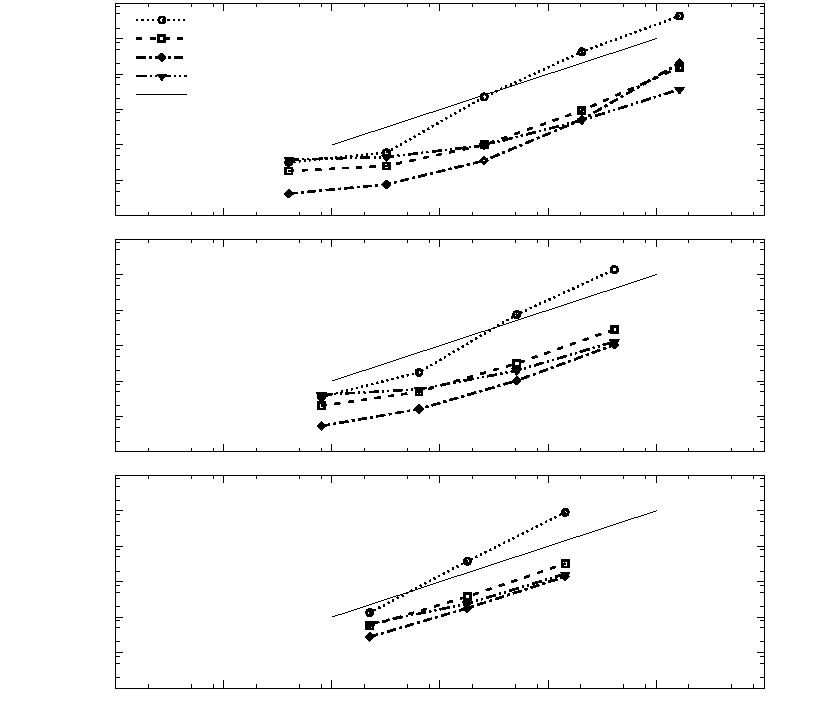
\includegraphics{ConstCoeffPoisson_Schwarz}}%
    \gplfronttext
  \end{picture}%
\endgroup
